\documentclass[french,11pt,twoside]{VcCours}
\newcommand{\dt}{\text{d}t}
\newcommand{\dx}{\text{d}x}

\renewcommand{\trou}[1]{{\color{white}#1}}
%\renewcommand{\trou}[1]{{\color{blue}#1}}

% cSpell:ignore orthonormalisons orthonormaliser 

\begin{document}

\Titre{PSI}{Promotion 2021--2022}{Mathématiques}{Chapitre 14 : Espaces préhilbertiens, espaces euclidiens}

\tableofcontents
\separationTitre


Dans ce chapitre, $H$ sera un $\mathbb{R}$-espace vectoriel et $n$ un entier supérieur ou égal à $1$.

\section{Produit scalaire}
\subsection{Définition}
\begin{Definition}{} Un \emph{produit scalaire} sur $H$ est une forme bilinéaire symétrique définie positive sur $H$, c'est-à-dire une application $\varphi : H \times H \rightarrow \mathbb{R}$ vérifiant les propriétés suivantes :

\begin{itemize}
\item \emph{Symétrie} : pour tout $(x,y) \in H^2$, $\varphi(x,y)= \varphi(y,x)$.
\item \emph{Bilinéarité} : pour tout $y \in H$, L'application 
$$ \begin{array}{ccl}
H & \rightarrow & \mathbb{R} \\
x & \mapsto & \varphi(x,y) \\
\end{array}$$
est linéaire. La symétrie implique alors la linéarité par rapport à la seconde variable.
\item \emph{Définie positivité} : pour tout $x \in H$, $\varphi(x,x) \geq 0$ et :
$$ \varphi(x,x) = 0 \Longleftrightarrow x = 0_H $$
\end{itemize}
\end{Definition}

\begin{Remarques}{}
\begin{itemize}
\item Si $\varphi$ est un produit scalaire sur $H$, on note souvent :
$$ \varphi(x,y) = <x,y>  \ou \varphi(x,y) = (x \vert y) \ou \varphi(x,y)=x \cdot y$$
\item Pour tout $x \in H$, $<x  \,  , \, 0_H > =<0_H  \,  , \, x > = 0$.
\end{itemize}
\end{Remarques}

\begin{Definition}{} 
\begin{itemize}
\item Si $H$ est muni d'un produit scalaire $\varphi$, on dit que $(H, \varphi)$ (ou plus simplement $H$ si il n'y a pas d'ambiguïté sur le produit scalaire) est un \emph{espace préhilbertien réel}.
\item Un\emph{ espace euclidien} est un espace préhilbertien réel de dimension finie.
\end{itemize}
\end{Definition}

\subsection{Exemples}

\textbf{Exemple 1 : Produit scalaire usuel sur $\mathbb{R}^n$}

Pour tout $x=(x_1, \ldots, x_n) \in \mathbb{R}^n$ et $y=(y_1, \ldots, y_n) \in \mathbb{R}^n$, on pose :
$$ \phantom{\fbox{$<x,y> \, = \sum_{i=1}^n x_i y_i $}}$$
Montrons que cela définit bien un produit scalaire sur $\mathbb{R}^n$ :

\vspace{6cm}

\newpage

% $\phantom{test}$

% \vspace{2cm}

\begin{Remarque}{} Soient $E$ un $\mathbb{R}$-espace vectoriel de dimension finie et $(e_1, \ldots, e_n)$ une base de $E$. Tout $x \in E$ et tout $y \in E$ s'écrivent alors de manière unique sous la forme :
$$ x = \sum_{k=1}^n x_k e_k \et  y = \sum_{k=1}^n y_k e_k$$
où $(x_1, \ldots, x_n) \in \mathbb{R}^n$ et $(y_1, \ldots, y_n) \in \mathbb{R}^n$. Alors si l'on pose :
$$ <x,y> \, = \sum_{i=1}^n x_i y_i$$
Cela définit un produit scalaire sur $E$ (preuve équivalente à celle effectuée précédemment).
\end{Remarque} 
\medskip

\textbf{Exemple 2 : Produit scalaire usuel sur $\mathcal{M}_{n,1}(\mathbb{R})$}

Pour toutes matrices colonnes $X, Y \in \mathcal{M}_{n,1}(\mathbb{R})$, on pose :
$$ \phantom{\fbox{$<X,Y> \, = ~^tX Y $}}$$
Remarquons que si $X = \begin{pmatrix}
x_1 \\
\vdots \\
x_n \\
\end{pmatrix}$ et $Y = \begin{pmatrix}
y_1 \\
\vdots \\
y_n \\
\end{pmatrix}$, on a :
$$ <X,Y> = (x_1, \ldots, x_n) \begin{pmatrix}
y_1 \\
\vdots \\
y_n \\
\end{pmatrix} = \sum_{i=1}^{n} x_i y_i $$
On retrouve donc le produit scalaire de l'exemple 1 (en identifiant $\mathbb{R}^n$ et $\mathcal{M}_{n,1}(\mathbb{R})$).

\medskip

\textbf{Exemple 3 : Produit scalaire usuel sur $\mathcal{M}_{n}(\mathbb{R})$}

Pour toutes matrices $A,B \in \mathcal{M}_n(\mathbb{R})$, on pose :
$$ \phantom{\fbox{$<A,B> = \textrm{Tr}(~^tA B)$}} $$
Montrons que cela définit un produit scalaire sur $\mathcal{M}_n(\mathbb{R})$ :


\vspace{6cm}

\newpage

\phantom{test}

\vspace{3cm}

\textbf{Exemple 4 : Produit scalaire sur $\mathcal{C}([a,b], \mathbb{R})$ où $a<b$}

Soit $\omega : [a,b] \rightarrow \mathbb{R}$ une fonction \emph{continue} et \emph{strictement positive} sur $[a,b]$. Pour toutes fonctions $f,g \in \mathcal{C}([a,b], \mathbb{R})$, on pose :
$$ \fbox{$<f,g> = \int_{a}^b f(x) g(x) \omega(x) \dx$}$$
Montrons que cela définit un produit scalaire sur $\mathcal{C}([a,b], \mathbb{R})$ :

\vspace{8.5cm}

\begin{Remarque}{} On obtient un produit scalaire classique en posant $ \omega : x \mapsto 1$.
\end{Remarque}

\begin{ApplicationDirecte}{} Posons pour tout $(P,Q) \in \mathbb{R}_n[X]^2$,
$$ <P,Q> = \sum_{k=0}^n P(k) Q(k) $$
Montrer que cela définit un produit scalaire sur $\mathbb{R}_n[X]$.
\end{ApplicationDirecte}

\subsection{Inégalité de Cauchy-Schwarz et inégalité triangulaire}
Dans la suite, sans mention particulière, $H$ désigne un espace préhilbertien réel muni d'un produit scalaire noté $< \cdot , \cdot>$.

\begin{Theoreme}{Inégalité de Cauchy-Schwarz} Pour tout $(x,y) \in H^2$, on a :
$$ \phantom{\vert <x,y> \vert \leq \sqrt{<x,x>} \sqrt{<y,y>}}$$
avec égalité si et seulement \phantom{si $x$ et $y$ sont colinéaires.}
\end{Theoreme}

\begin{Demonstration}{}

\vspace{15cm}
\end{Demonstration}

% \newpage

% $\phantom{test}$

% \vspace{9cm}

\begin{TheoremeDefinition}{} On pose pour tout $x \in H$,
$$ \Vert x \Vert = \sqrt{<x,x>}$$
\begin{itemize}
\item L'application $\Vert \cdot \Vert : H \rightarrow \mathbb{R}$ est alors une norme sur $H$ que l'on appelle \emph{norme euclidienne}.
\item Pour tout $(x,y) \in H^2$, on pose $\textrm{d}(x,y) = \Vert x-y \Vert$. L'application $d$ est appelée \emph{distance euclidienne} associée à $\Vert \cdot \Vert$.
\end{itemize}
\end{TheoremeDefinition} 

\begin{Demonstration}{} Effectuée dans le chapitre sur les espaces normés.
%
%\vspace{7.5cm}
\end{Demonstration}

\begin{Theoreme}{Cas d'égalité dans l'inégalité triangulaire}
Considérons un produit scalaire $< \cdot , \cdot>$ sur $H$ et notons $\Vert \cdot \Vert$ la norme euclidienne associée. Pour tout $(x,y) \in H^2$, on a l'équivalence suivante :
$$ \Vert x+y \Vert = \Vert x \Vert + \Vert y \Vert \Longleftrightarrow \exists \alpha \in \mathbb{R}_{+} \, / x= \alpha y \hbox{ ou } y = \alpha x $$
\end{Theoreme}

\begin{Demonstration}{} 

\vspace{8.5cm}

\vspace{\stretch{1}}
\end{Demonstration}

\newpage

% \phantom{test}

% \vspace{5cm}

\begin{Remarque}{} Pour tout $(x,y) \in H^2$,
$$ \Vert x+y \Vert^2 = \phantom{testetstststtestetststststststststst}$$
et
$$ \Vert x-y \Vert^2 =  \phantom{testetstststtestetststststststststst}$$
\end{Remarque}


\begin{center}
\textbf{Petite synthèse.}
\end{center}

\begin{tabular}{|c|c|c|c|c|}
\hline
Espace & Produit scalaire usuel & Norme associée & Inégalité de Cauchy-Schwarz & Inégalité triangulaire \\
\hline
& & & & \\
& & & & \\
& & & & \\
& & & & \\
& & & & \\
& & & & \\
\hline
& & & & \\
& & & & \\
& & & & \\
& & & & \\
& & & & \\
& & & & \\
\hline
& & & & \\
& & & & \\
& & & & \\
& & & & \\
& & & & \\
& & & & \\
\hline
& & & & \\
& & & & \\
& & & & \\
& & & & \\
& & & & \\
& & & & \\
\hline
\end{tabular}



\begin{Exemple}{} Soit $(x_1, \ldots, x_n) \in \mathbb{R}^n$. Montrons que :
$$ \left(\sum_{i=1}^n x_i \right)^2 \leq n \sum_{i=1}^n x_i^2$$
Quand a t-on égalité ?

%\vspace{6cm}

\end{Exemple}

\newpage

\begin{ApplicationDirecte}{} Soit $f : [0,1] \rightarrow \mathbb{R}$ une fonction continue et positive. On pose pour tout $n \geq 0$,
$$ I_n = \int_{0}^1 t^n f(t) \dt$$
Montrer que pour tout $(p,q) \in \mathbb{N}^2$,  $I_{n+p}^2 \leq I_{2n} I_{2p}$.
\end{ApplicationDirecte}

\subsection{Deux identités}
Dans la suite, sans mention particulière, $H$ désigne un espace préhilbertien réel muni d'un produit scalaire $< \cdot , \cdot>$ et on note $\Vert \cdot \Vert$ la norme euclidienne associée.

\begin{Proposition}{Identités de polarisation} Pour tout $(x,y) \in H^2$, on a :
\begin{align*}
<x,y> & = \frac{1}{2} ( \Vert x+ y \Vert^2 - \Vert x \Vert^2 - \Vert y \Vert^2 )  \\
%& = \frac{1}{2} ( \Vert x \Vert^2 + \Vert y \Vert^2 - \Vert x-y \Vert^2) \\
& = \frac{1}{4} ( \Vert x+y \Vert^2 - \Vert x-y \Vert^2) 
\end{align*}
\end{Proposition}

\begin{Demonstration}{} 

\vspace{6cm}
\end{Demonstration}

\begin{Remarque}{} La norme euclidienne associée à un produit scalaire est définie à l'aide de celui-ci. Les identités de polarisation montrent que si l'on connaît la norme euclidienne associée à un produit scalaire, on peut retrouver celui-ci.
\end{Remarque}

\begin{Proposition}{Identité du parallélogramme}
Considérons un produit scalaire $< \cdot , \cdot>$ sur $H$ et notons $\Vert \cdot \Vert$ la norme euclidienne associée. Pour tout $(x,y) \in H^2$, on a :
$$ \Vert x+y \Vert^2 + \Vert x-y \Vert^2 = 2 (\Vert x \Vert^2 + \Vert y \Vert^2)$$
\end{Proposition}

\newpage
\begin{center}
\textbf{Représentation graphique.}
\end{center}

\vspace{3cm}

\begin{Demonstration}{}

  \vspace{3cm}
\end{Demonstration}

\section{Orthogonalité}
Dans tout le paragraphe, on considère un produit scalaire $< \cdot , \cdot>$ sur $H$ et on note $\Vert \cdot \Vert$ la norme euclidienne associée.

\subsection{Définitions et premières propriétés}

\begin{Definition}{} Soient $x,y \in H$.
\begin{itemize}
\item On dit que $x$ et $y$ sont \emph{orthogonaux}, et on note $x \perp y$, si $<x,y>=0$.
\item On dit que $x$ est \emph{unitaire} si $\Vert x \Vert =1$.
\end{itemize}
\end{Definition}

\begin{Definition}{} Soit $(x_i)_{i \in I}$ une famille de vecteurs de $H$ ($I$ est un ensemble d'indices). On dit que cette famille est :
\begin{itemize}
\item \emph{normée} si pour tout $i \in I$, $\Vert x_i \Vert=1$.
\item \emph{orthogonale} si pour tout $(i,j) \in I^2$ tel que $i \neq j$, $<x_i ,x_j>=0$.
\item \emph{orthonormale} si elle est orthogonale et normée.
\end{itemize}
\end{Definition}

\begin{Remarques}{}
\begin{itemize}
\item Si un vecteur $x$ de $H$ est non nul alors $y = \dfrac{x}{\Vert x \Vert}$ est unitaire :

\vspace{2cm}
\item $(x_i)_{i \in I}$ est orthonormale si et seulement si : $\forall (i,j) \in I^2$, $<x_i,x_j>= \delta_{i,j}$.
\end{itemize}
\end{Remarques}

\begin{Proposition}{} Une famille orthogonale finie de vecteurs non nuls de $H$ est libre.
\end{Proposition}

\begin{Demonstration}{}
\vspace{5cm}
\end{Demonstration}

\begin{ApplicationDirecte}{} Notons pour tout $k \in \mathbb{N}$, $f_k : x \mapsto \cos(kx)$. Calculer pour tout $(p,q) \in \mathbb{N}^2$,
$$ \int_{0}^{2 \pi} \cos(px) \cos(qx) \dx$$
En déduire que pour tout $n \geq 0$, $(f_0, \ldots, f_n)$ est une famille libre de $\mathcal{C}^0([0,2 \pi],\mathbb{R})$.
\end{ApplicationDirecte}

\begin{Theoreme}{Pythagore}
Pour tout $(x,y) \in H^2$, on a :
$$ \Vert x+y \Vert^2 = \Vert x \Vert^2 + \Vert y \Vert^2 \Longleftrightarrow x \perp y $$
\end{Theoreme}

\begin{Demonstration}{}
\vspace{3cm}
\end{Demonstration}

\begin{Remarque}{} Soient $x_1, \ldots, x_n$ des vecteurs deux à deux orthogonaux de $H$. Alors :
$$ \Vert x_1 + \cdots + x_n \Vert^2 = \phantom{blablablablablablablablablabla}$$

\vspace*{2cm}~

\end{Remarque}

\subsection{Bases orthonormées et orthonormalisation}
\begin{Definition}{} Soient $H$ un espace euclidien et $B= (e_1, \ldots, e_n)$ une famille de vecteurs de $H$. On dit que $\mathcal{B}$ est une base \emph{orthonormée} de $H$ si $\mathcal{B}$ est une base et une famille orthonormale de $H$.
\end{Definition}

\begin{Exemple}{} La base canonique de $\mathbb{R}^n$ est une base orthonormée pour le produit scalaire usuel.
\end{Exemple}

\begin{Proposition}{Calcul dans une base orthonormée}
Soient $H$ un espace euclidien et $\mathcal{B}=(e_1, \ldots, e_n)$ une base orthonormée de $H$.

Soient $x,y \in H$. Il existe deux uniques $n$-uplets de réels $(x_1, \ldots, x_n)$ et $(y_1, \ldots, y_n)$ tels que :
$$ x = \sum_{i=1}^n x_i e_i \et y = \sum_{i=1}^n y_i e_i $$
Alors on a :
$$ <x,y> = \sum_{i=1}^n x_i y_i \et  \Vert x \Vert = \left( \sum_{i=1}^n x_i^2 \right)^{1/2} $$
\end{Proposition}

\begin{Demonstration}{}
\vspace{4cm}
\end{Demonstration}

\begin{Remarques}{}
\begin{itemize} 
\item L'intérêt de travailler dans une base orthonormée est de pouvoir utiliser uniquement les coordonnées pour déterminer un produit scalaire ou une norme.
\item Si on note $X$ et $Y$ les vecteurs colonnes des coordonnées de $x$ et $y$ dans la base $\mathcal{B}$, on a :
$$ <x,y> = ~^tXY \et \Vert X \Vert = (~^tXX)^{1/2}$$
\end{itemize}
\end{Remarques}

\begin{Proposition}{Matrice d'un endomorphisme dans une base orthonormée}
Soient $H$ un espace euclidien et $\mathcal{B}=(e_1, \ldots, e_n)$ une base orthonormée de $H$. Si $u$ est un endomorphisme de $H$ alors :
$$ \textrm{Mat}_{\mathcal{B}}(u) = (<e_i, u(e_j)>)_{1 \leq i,j \leq n}$$
\end{Proposition}

\begin{Demonstration}{}
\vspace{6cm}
\end{Demonstration}


\begin{Theoreme}{Procédé d'orthonormalisation de Gram-Schmidt}
Soient $p \geq 1$, $(e_1, \ldots, e_p)$ une famille libre de vecteurs de $H$ et $F = \Vect(e_1, \ldots, e_p)$. Alors il existe une base orthonormée $(\varepsilon_1, \ldots, \varepsilon_p)$ de $F$ telle que pour tout $i \in \ii{1}{p}$,
$$ \Vect(\varepsilon_1, \ldots, \varepsilon_i) = \Vect(e_1, \ldots, e_i) $$
\end{Theoreme}
%
%\begin{Demonstration}{}
%\vspace{10cm}
%\end{Demonstration}

\begin{Remarques}{}
\begin{itemize}
\item Si l'on impose la condition $<\varepsilon_i, e_i>  >0$ pour tout $i$, la famille $(\varepsilon_1, \ldots, \varepsilon_p)$ est alors unique.
\item La démonstration admise est constructive : elle donne un algorithme (détailler ensuite) qui permet de construire cette nouvelle famille. On remarque que l'on peut décider de normer les vecteurs à la fin de l'algorithme : ceci permet d'éviter des erreurs de calculs.
\end{itemize}
\end{Remarques}

\medskip

\begin{center}
\textbf{Méthode pratique d'orthonormalisation d'une famille $(e_1, \ldots, e_p)$.}
\end{center}

\begin{itemize}
\item On pose $f_1=e_1$.
\item On choisit $f_2$ de la forme $e_2+ \alpha f_1$ ($\alpha \in \mathbb{R}$) de sorte que $<f_2, f_1>=0$.
\item On choisit $f_3$ de la forme $e_3 + \alpha f_1 + \beta f_2$ de sorte que $<f_3,f_1>=0$ et $<f_3,f_2>=0$.
\item Ainsi de suite pour trouver $f_4, \ldots, f_p$.
\item On calcule la norme des vecteurs $f_i$ pour $i \in \ii{1}{p}$ et on pose $\varepsilon_i = \dfrac{f_i}{\Vert f_i \Vert} \cdot$
\end{itemize}

\medskip

\begin{Exemple}{} Posons $x_1= (1,1,0)$, $x_2=(0,1,1)$ et $x_3=(1,0,1)$. Montrons que $(x_1,x_2,x_3)$ est une base de $\mathbb{R}^3$ (muni du produit scalaire usuel) et orthonormalisons la.

\newpage

\vspace*{5cm}
\end{Exemple}


\begin{Exemple}{} Soit $\mathcal{B}=(1,X,X^2)$ la base canonique de $\mathbb{R}_2[X]$ muni du produit scalaire défini par :
$$ \forall (P,Q) \in \mathbb{R}_2[X]^2, \; <P,Q> = \int_{0}^1 P(t) Q(t) \dt $$
Orthonormalisons la base $\mathcal{B}$.

\vspace{10cm}
\end{Exemple}

\begin{ApplicationDirecte}{} Considérons $\mathbb{R}^3$ muni du produit scalaire usuel et notons $\mathcal{B}=(e_1,e_2,e_3)$ sa base canonique. Vérifier que $\mathcal{B}'= (e_1+e_2+e_3, e_1-e_2+e_3, e_1+e_2-e_3)$ est une base de $\mathbb{R}^3$ et orthonormaliser-la.
\end{ApplicationDirecte}

\begin{Corollaire}{} Tout espace euclidien $H$ admet une base orthonormée et tout famille orthonormée d'un espace euclidien $H$ peut être complétée en une base orthonormée de $H$.
\end{Corollaire}

\begin{Demonstration}{}
\vspace{5cm}
\end{Demonstration}


\subsection{Somme et orthogonalité}

\begin{Definition}{} Soient $F$ et $G$ deux sous-espace vectoriel de $H$. On dit que $F$ et $G$ sont \emph{orthogonaux} si :
$$ \phantom{\forall (f,g) \in F \times G, \; <f,g>=0}$$
On note dans ce cas : $F \perp G$.
\end{Definition}

\begin{TheoremeDefinition}{} Soient $p \geq 1$ et $F_1, \ldots, F_p$ des sous-espaces vectoriels de $H$ deux à deux orthogonaux. Alors la somme $F_1 + \cdots + F_p$ est directe.

On appelle alors la somme $F_1 \oplus \cdots \oplus F_p$ la \emph{somme directe orthogonale} des $F_i$ et on dit que les $F_i$ sont en \emph{somme directe orthogonale}.
\end{TheoremeDefinition}

\begin{Demonstration}{}

\vspace{5cm}
\end{Demonstration}

\begin{Definition}{} Soient $F$ et $G$ deux sous-espace vectoriels de $H$. On dit que $F$ et $G$ sont \emph{supplémentaires orthogonaux} si $F \perp G$ et $H=F \oplus G $. On note alors $H= F \overset{\perp}{\oplus} G$.
\end{Definition}

\begin{Remarque}{} On sait qu'une somme de sous-espaces deux à deux orthogonaux est nécessairement directe. Ainsi pour deux sous-espaces $F$ et $G$ d'un espace préhilbertien réel $H$ : 
$$H= F \overset{\perp}{\oplus} G  \Longleftrightarrow  H = F+G \et F \perp G$$
\end{Remarque}

\subsection{Orthogonal d'un sous-espace vectoriel}

\begin{TheoremeDefinition}{} Soit $F$ un sous-espace vectoriel de $H$. On appelle \emph{orthogonal} de $F$ et on note $F^{\perp}$ l'ensemble défini par :
$$ \phantom{F^{\perp} = \lbrace y \in H \, \vert \, \forall x \in F, \, <x,y>=0 \rbrace}$$
C'est un sous-espace vectoriel de $H$, orthogonal à $F$.
\end{TheoremeDefinition}

\begin{Demonstration}{}

\vspace{6cm}
\end{Demonstration}

\begin{Proposition}{} $H^{\perp} = \lbrace 0_H \rbrace$ et $\lbrace 0_H \rbrace^{\perp} = H$.
\end{Proposition}

\begin{Demonstration}{}
\vspace{2cm}
\end{Demonstration}

\begin{ApplicationDirecte}{} Soient $x,y \in H$ tels que pour tout $z \in H$, $<x,z>=<y,z>$. Que peut-on en déduire ?
\end{ApplicationDirecte}

\begin{Proposition}{} Soient $F$ un sous-espace vectoriel de dimension finie de $H$ et $(e_1, \ldots, e_p)$ une famille génératrice de $F$ ($p \geq 1$). Pour tout $x \in H$, on a :
$$ x \in F^{\perp} \Longleftrightarrow \forall i \in \ii{1}{p}, \, <x,e_i> =0 $$
\end{Proposition}

\begin{Demonstration}{}
\vspace{6cm}

\vspace{\stretch{1}}
\end{Demonstration}

\begin{Proposition}{} Soit $F$ un sous-espace vectoriel de $H$. Alors :
\begin{itemize}
\item $F \subset (F^{\perp})^{\perp}$.
\item $F$ et $F^{\perp}$ sont en somme directe orthogonale (en particulier $F \cap F^{\perp} = \lbrace 0_H \rbrace$).
\item Si $G$ est un supplémentaire orthogonal de $F$ alors $G= F^{\perp}$.
\end{itemize}
\end{Proposition}

\begin{Demonstration}{}

\vspace{6cm}
\vspace{\stretch{1}}
\end{Demonstration}

\begin{Remarque}{} Attention l'inclusion réciproque du premier point est fausse en général et les espaces $F$ et $F^{\perp}$ ne sont pas forcément supplémentaires dans $H$ (voir TD pour un exemple).
\end{Remarque}

\newpage

\begin{Theoreme}{Supplémentaire orthogonal d'un sev de dimension finie}
Soit $F$ un sous-espace vectoriel de \emph{dimension finie} de $H$. Alors :
\begin{itemize}
\item $H = F \oplus F^{\perp}$.
\item $(F^{\perp})^{\perp}=F$.
\end{itemize}
\end{Theoreme}

\begin{Demonstration}{}
\vspace{9cm}

\vspace{\stretch{1}}


\end{Demonstration}

\begin{Theoreme}{Projection orthogonale} Soit $F$ un sous-espace vectoriel de dimension finie de $H$. On sait que $F \oplus F^{\perp}=H$ donc la projection $p_F$ sur $F$ parallèlement à $F^{\perp}$ est bien définie et est appelée \emph{projection orthogonale} sur $F$.

Si $(\varepsilon_1, \ldots, \varepsilon_p)$ est une base orthonormée de $F$ alors pour tout $x \in H$,
$$ p_F(x) = \sum_{i=1}^p <x, \varepsilon_i> \varepsilon_i $$
Le vecteur $p_F(x)$ est appelé le \emph{projeté orthogonal} de $x$ sur $F$.
\end{Theoreme}


On a donc deux méthodes pour déterminer l'expression de $p_F(x)$ :
\begin{itemize}
\item On détermine une base orthonormée de $F$ (en utilisant l'algorithme de Gram-Schmidt par exemple) et on utilise la formule précédente.
\item On remarque que $p_F(x)$ et l'unique élément $y$ de $F$ tel que $x-y \in F^{\perp}$ et on sait que si $(e_1, \ldots, e_p)$ est une famille génératrice de $F$ :
$$ x-y \in F^{\perp} \Longleftrightarrow \forall i \in \ii{1}{p}, \; <x-y, e_i>=0 $$
L'avantage  de cette méthode c'est qu'il n'y a pas besoin d'orthonormaliser une base.
\end{itemize}

\newpage
\begin{Exemple}{} Soient $H= \mathbb{R}^3$ muni du produit scalaire usuel et $D= \left\lbrace (x,y,z) \in \mathbb{R}^3 \, \vert \, x= \dfrac{y}{2} = \dfrac{z}{3} \right\rbrace \cdot$

Déterminons la matrice de la projection orthogonale sur $D$.

\vspace{10cm}
\end{Exemple}

\begin{ApplicationDirecte}{} Soient $H= \mathbb{R}^3$ muni du produit scalaire usuel et $P = \lbrace (x,y,z) \in \mathbb{R}^3 \, \vert \, x-2y+z=0 \rbrace \cdot$
Déterminer la matrice de la projection orthogonale sur $P$.
\end{ApplicationDirecte}

\begin{Proposition}{} Soit $\mathcal{B}= (\varepsilon_1, \ldots, \varepsilon_n)$ une base orthonormée d'un espace euclidien $H$. Alors la décomposition de tout vecteur $x$ de $H$ dans la base $\mathcal{B}$ est :
$$ x = \sum_{i=1}^n <x, \varepsilon_i> \varepsilon_i $$
\end{Proposition}

\begin{Demonstration}{} C'est une conséquence directe du théorème précédent en posant $F=H$ (le projeté de $x$ sur $F$ est alors lui-même).
\end{Demonstration}

\begin{Remarque}{} Si $(\varepsilon_1, \ldots, \varepsilon_n)$ est une base orthonormée de $H$, pour tous $x,y \in H$, on a :
$$ <x,y> = \sum_{i=1}^n <x,\varepsilon_i><y,\varepsilon_i> \et \Vert x \Vert = \left(\sum_{i=1}^n <x,\varepsilon_i>^2 \right)^{1/2}$$
\end{Remarque}

\begin{Proposition}{} Soit $F$ un sous-espace vectoriel d'un espace euclidien $E$. Alors $E= F \oplus F^{\perp}$ et en particulier :
$$   \textrm{dim}(E) = \textrm{dim}(F) + \textrm{dim}(F^{\perp})$$
\end{Proposition}

\begin{Remarque}{} On peut aussi définir la \emph{symétrie orthogonale} par rapport à $F$ qui n'est rien d'autre que la symétrie par rapport à $F$ parallèlement à $F^{\perp}$. Si $F$ est un hyperplan, on dit que cette symétrie est la \emph{réflexion} par rapport à $F$.
\end{Remarque}

\section{Distance à un sous-espace}

\emph{Problématique} : Soient $x$ un vecteur de $H$ et $F$ un sous-espace vectoriel de $H$. Existe t-il un vecteur de $F$ qui soit \og le plus proche \fg de $x$ au sens de la distance associée au produit scalaire ? Si oui, comment le déterminer ?

\medskip

\begin{Theoreme}{} Soient $x$ un vecteur de $H$ et $F$ un sous-espace vectoriel de $H$ de \emph{dimension finie}. L'ensemble 
$$ \lbrace \Vert x-y \Vert \, \vert \, y \in F \rbrace$$
admet un minimum, celui-ci est atteint en un unique vecteur qui est $p_F(x)$. Ainsi :
$$ \Vert x - p_F(x) \Vert = \min_{y \in F} \Vert x-y \Vert$$
Le réel positif $\Vert x - p_F(x) \Vert$ est appelé \emph{distance} de $x$ à $F$ et est noté $\textrm{d}(x,F)$. Ainsi :
$$ \textrm{d}(x,F) = \Vert x - p_F(x) \Vert = \min_{y \in F} \Vert x-y \Vert$$
\end{Theoreme}

\begin{center}
\textbf{Illustration graphique de la notion de distance.}
\end{center}

\begin{center}
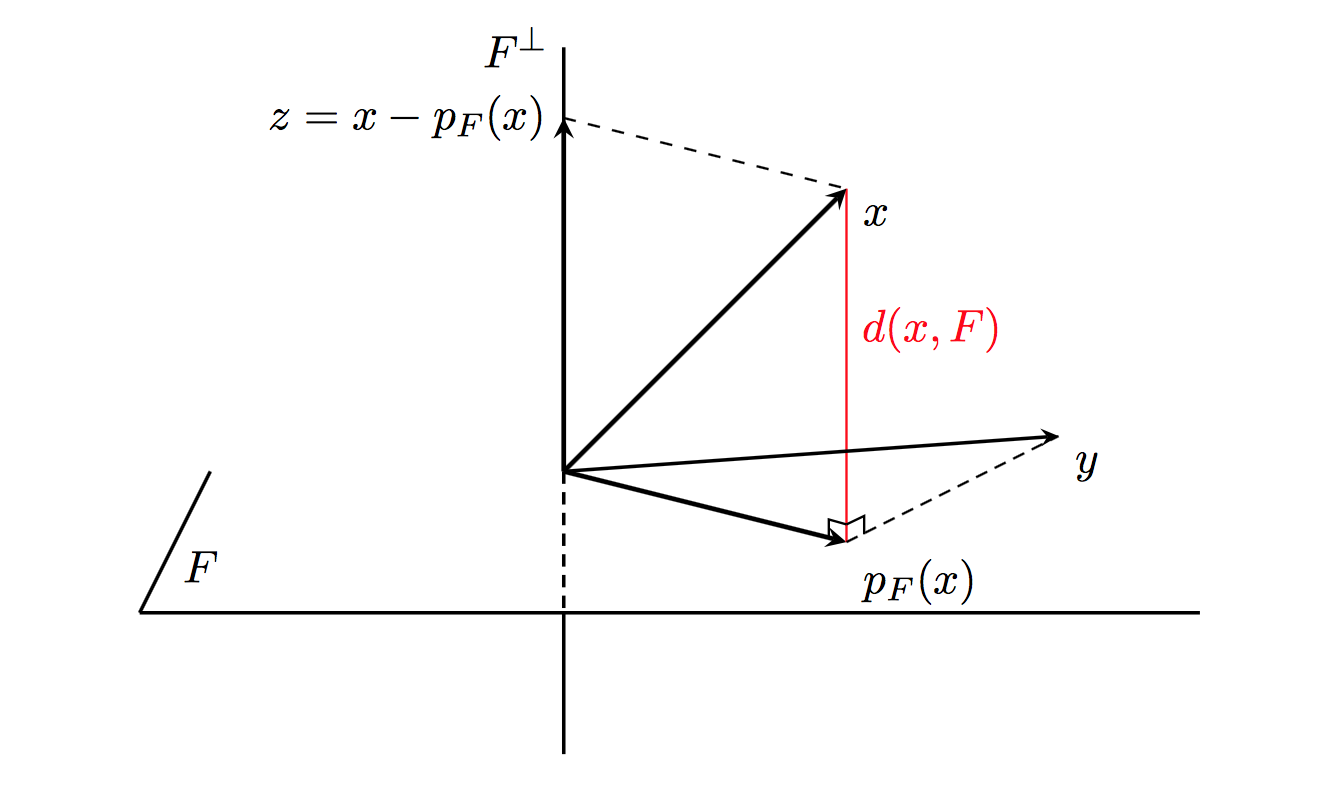
\includegraphics[scale=0.4]{dist}
\end{center}

\begin{Demonstration}{}

\newpage

\vspace*{4cm}
\end{Demonstration}

\begin{Proposition}{} Soient $F$ un sous-espace vectoriel de dimension finie de $H$ et $(\varepsilon_1, \ldots, \varepsilon_n)$ une base orthonormée de $F$. Alors :
$$ \textrm{d}(x,F)^2 = \Vert x \Vert^2 - \Vert p_F(x) \Vert^2 = \Vert x \Vert^2 - \sum_{i=1}^n <x,\varepsilon_i>^2 $$
\end{Proposition}

\begin{Demonstration}{}
\vspace{6cm}
\end{Demonstration}


\begin{Exemple}{} Déterminons $\inf_{(a,b) \in \mathbb{R}^2} \int_{0}^1 (t^2-(at+b))^2 \dt$.

\newpage

\vspace*{3cm}
\end{Exemple} 

\begin{Corollaire}{Inégalité de Bessel}
Soient $F$ un sous-espace vectoriel de dimension finie de $H$. Pour tout $x \in H$, on a :
$$ \Vert p_F(x) \Vert \leq \Vert x \Vert$$
En particulier si $(\varepsilon_1, \ldots, \varepsilon_p)$ est une famille orthonormale de $F$,
$$ \sum_{i=1}^p <x,\varepsilon_i>^2 \leq \Vert x \Vert^2 $$
\end{Corollaire}

\begin{Demonstration}{}
\vspace{2cm}
\end{Demonstration}

\begin{ApplicationDirecte}{} 
  On munit $E = \mathcal{C}([ - 1,1],\mathbb{R})$ du produit scalaire:
  \[
  <f,g> = \frac{1}{2}\int_{ - 1}^{1} f(x)g(x) \dx
  \]
Pour $i \in \ii{0}{3}$, on pose $P_{i} : x \mapsto x^{i}$.
  \begin{enumerate}
  \item Montrer que la famille $(P_{0} ,P_{1} ,P_{2})$ est libre mais pas orthogonale.
  \item Déterminer, par le procédé de Gram-Schmidt, une base orthonormée $(Q_{0} ,Q_{1} ,Q_{2})$ de l'espace $F = \Vect(P_{0} ,P_{1} ,P_{2})$ à partir de la famille $(P_{0} ,P_{1} ,P_{2})$.
  \item Calculer la projection orthogonale de $P_{3}$ sur $F$ puis déterminer la distance de $P_{3}$ à $F$.
  \end{enumerate}
\end{ApplicationDirecte}

\section{Formes linéaires}
Dans cette section, $H$ désigne un espace euclidien muni d'un produit scalaire $< \cdot, \cdot>$.

\begin{Theoreme}{} Soit $f$ une forme linéaire sur $H$. Il existe un unique vecteur $a \in H$ tel que pour tout $x \in H$,
$$ f(x)= <a,x>$$
\end{Theoreme}

\begin{Demonstration}{}
\vspace{4cm}

\vspace{\stretch{1}}

\end{Demonstration}

\begin{Exemples}{}
\begin{enumerate}
\item Considérons $\mathbb{R}^3$ muni du produit scalaire usuel. Posons pour tout $(x,y,z) \in \mathbb{R}^3$,
$$ f((x,y,z)) = x+y+2z $$
Il est facilement de voir que :
$$ f((x,y,z)) = <(1,1,2), (x,y,z)>$$
\item Les formes linéaires de $\mathcal{M}_n(\mathbb{R})$ sont de la forme :
$$ M \mapsto \textrm{Tr}(~^tA M) $$
où $A \in \mathcal{M}_n(\mathbb{R})$.
\end{enumerate}
\end{Exemples}

\begin{Definition}{} Soient $H$ un espace euclidien, $P$ un hyperplan de $H$ et $f$ une forme linéaire telle que $P = \textrm{Ker}(f)$. D'après le théorème précédent, il existe alors un unique vecteur $a$ de $E$ tel que pour tout $x \in H$, 
$$ f(x) = <a,x>$$
Ainsi pour tout $x \in E$, on a :
$$ x \in P \Longleftrightarrow <x,a>= 0$$
On dit que $a$ est un \emph{vecteur normal} à $P$.

Si $\mathcal{B}=(\varepsilon_1, \ldots, \varepsilon_n)$ est une base orthonormée de $H$. Si $(x_1, \ldots, x_n)$ sont les coordonnées de $x$ dans la base $\mathcal{B}$ et si $(a_1, \ldots, a_n)$ sont les coordonnées de $a$ dans la base $\mathcal{B}$ alors on a :
$$ <a,x> = a_1 x_1 + \cdots + a_n x_n $$
et ainsi $P$ a pour équation :
$$ a_1 x_1 + \cdots + a_n x_n = 0$$
dans la base $\mathcal{B}$. 
\end{Definition}

\newpage

\begin{Proposition}{Distance d'un vecteur à un hyperplan ou une droite}
Soit $H$ un espace euclidien.
\begin{itemize}
\item Soient $P$ un hyperplan de $H$ et $a$ un vecteur normal à $P$. Alors, pour tout $x \in H$, la distance de $x$ à $P$ est donnée par :
$$ \textrm{d}(x,P) = \dfrac{\vert <x,a> \vert}{\Vert a \Vert}$$
\item Soient $D$ une droite vectorielle de $H$ et $a$ un vecteur non nul de $D$. Alors, pour tout $x \in H$, la distance de $x$ à $D$ est donnée par :
$$ \textrm{d}(x,D) = \sqrt{\Vert x \Vert^2 -  \dfrac{\vert <x,a> \vert^2}{\Vert a \Vert^2}} $$
\end{itemize}
\end{Proposition}

\begin{Demonstration}{}
\vspace{8.5cm}
\end{Demonstration}

\begin{Exemple}{} Soient $H = \mathcal{M}_2(\mathbb{R})$ et $T$ l'ensemble des matrices de $H$ de trace nulle. Déterminer la distance de $A = \begin{pmatrix}
1 & 2 \\
3 & 4 \\
\end{pmatrix}$ à $T$.

\end{Exemple}

\newpage

$\phantom{test}$

\vspace{2cm}


\begin{ApplicationDirecte}{} Soit $\mathbb{R}^3$ muni du produit scalaire usuel. Déterminer la distance de $(1,1,1)$ à 
$$P = \lbrace (x,y,z) \in \mathbb{R}^3 \, \vert \, x+y+z=0 \rbrace$$
 et à $D$, la droite vectorielle engendrée par $(1,1,1)$.
\end{ApplicationDirecte}

\section{Quelques compléments}
\subsection{Un peu de géométrie dans \texorpdfstring{$\mathbb{R}^2$ et $\mathbb{R}^3$}{ℝ² et ℝ³}}
\begin{Exemple}{} Considérons $\mathbb{R}^2$ muni du produit scalaire usuel. Déterminons l'équation de la droite passant par $(1,2)$ et orthogonal à $(1,1)$.

\vspace{3cm}
\end{Exemple}

\begin{Exemple}{} Considérons $\mathbb{R}^3$ muni du produit scalaire usuel. Déterminons l'équation du plan passant par $(1,1,1)$ et orthogonal à $(1,2,3)$.

\vspace{3cm}
\end{Exemple}

\subsection{Espaces fonctionnels}
Soient $I$ un intervalle de $\mathbb{R}$ non vide et non réduit à un point. L'ensemble $\mathbb{K}$ désignera $\mathbb{R}$ ou $\mathbb{C}$.

\begin{Definition}{} 
\begin{itemize}
\item On note $L^1(I, \mathbb{K})$ l'ensemble des fonctions continues par morceaux et intégrables sur $I$ et à valeurs dans $\mathbb{K}$.
\item On note $L^2(I, \mathbb{K})$ l'ensemble des fonctions $f : I \rightarrow \mathbb{K}$ continues par morceaux et telles que $\vert f \vert^2$ soit intégrable sur $I$ (on dit que $f$ est de \emph{carré intégrable} sur $I$).
\end{itemize}
\end{Definition}

\begin{Proposition}{} L'ensemble $L^1(I, \mathbb{K})$ est un $\mathbb{K}$-espace vectoriel.
\end{Proposition}

\begin{Demonstration}{} 

\vspace{6.5cm}
\end{Demonstration}

\begin{Remarque}{} Si $f : I \rightarrow \mathbb{K}$ et \emph{continue} et intégrable sur $I$ et si :
$$ \int_{I} \vert f(t) \vert \dt =0$$
alors $f$ est nulle sur $I$.
\end{Remarque}

\begin{Proposition}{} 
\begin{itemize}
\item Le produit de deux éléments de $L^2(I, \mathbb{K})$ est un élément de $L^1(\mathbb{K})$.
\item L'ensemble $L^2(I, \mathbb{K})$ est un $\mathbb{K}$-espace vectoriel.
\end{itemize}
 \end{Proposition}
 
 \begin{Demonstration}{}
 \vspace{8.5cm}
 \end{Demonstration}
 
 \begin{Proposition}{} Posons $H = \mathcal{C}(I, \mathbb{R}) \cap L^2(I, \mathbb{R})$. On pose pour tout $(f,g) \in H^2$,
 $$ <f,g> = \int_{I} fg$$
Alors cela définit un produit scalaire sur $H$.
 \end{Proposition}
 
 
\begin{Demonstration}{}
 
 \vspace{4cm}
 \end{Demonstration}
 
\begin{Remarque}{} La norme associée dans ce cas est alors définie par :
$$ \forall f \in H, \; \Vert f \Vert = \left( \int_{I} f^2 \right)^{1/2} $$
et on a l'inégalité de Cauchy-Schwarz suivante :
$$ \forall (f,g) \in H^2, \; \left\vert \int_{I} fg  \right\vert \leq  \Vert f \Vert \, \Vert g \Vert $$
\end{Remarque}
\end{document}
